\setchapterimage[2cm]{../images/header-introduction.jpg}
%\setchapterpreamble[u]{\margintoc}
\chapter{Introduction}
\labch{introduction}

While this study is narrated using real, specific molecular systems, it's actually a work about methodologies, techniques and their development.
Its flow focuses around a certain toxin and a family of molecules that may help identify it, but it has a more generic message: it aims to explain and showcase the fundamentals and applications of a variety of computational techniques that could be applied to a variety of systems.
This doesn't mean that the molecules of choice are any less important, as they have been researched by the author for a long time even before the drafting of this text, and have plenty of interest on their own.

\section{Marine toxins and saxitoxin}

The one molecule that initially motivated this work is the marine toxin saxitoxin.
\q{Marine toxins} is a loose term that groups several families of harmful substances produced by aquatic organisms such as phytoplanktons, dinoflagellates, algae, sponges, cnidarians, echinoderms, worms and fish.\sidecite{visciano16}
These toxins, usually part of the defense mechanisms of a certain species, can become actively dangerous to other organisms outside their food web when their populations increases disproportionally.

This is, precisely, the case of harfmul algal blooms.\sidenote{Some of them are known as \q{red tides}, due to the characteristic color that certain microorganisms can impart to seawater. However, only \num{300} in about \num{5000} marine species are colored, and most of them are not dangerous.\cite{wiley08}}
These algal blooms can occur due to changes in the usual ecosystem of toxin-producing species such as increases in the temperature of the water, or sudden raises in the availability of nutrients (e.g. due to a spill that includes nitrogen-rich compounds) that result in massive increases in their population.\cite{michalak13,chakraborty10,gobler17}
While the individual organisms may continue producing and emitting their toxins at their usual rates, the great increase in their population results in much higher concentrations of said toxins in the vicinity of their colonies.
Organisms that feed by filtering seawater start retaining and accumulating the toxins in their bodies.\cite{oikawa05}
This process of bioconcentration, which doesn't affect the health of the filterers,\sidecite{wiley08} turns them into dangerous reservoirs of toxin that, unmonitored, can turn into a danger to public health, as step by step these harmful substances end up reaching higher places in the food chain as exemplified in \reffig{food-chain}.\sidecite{gerssen10}

\begin{figure}
    \centering
    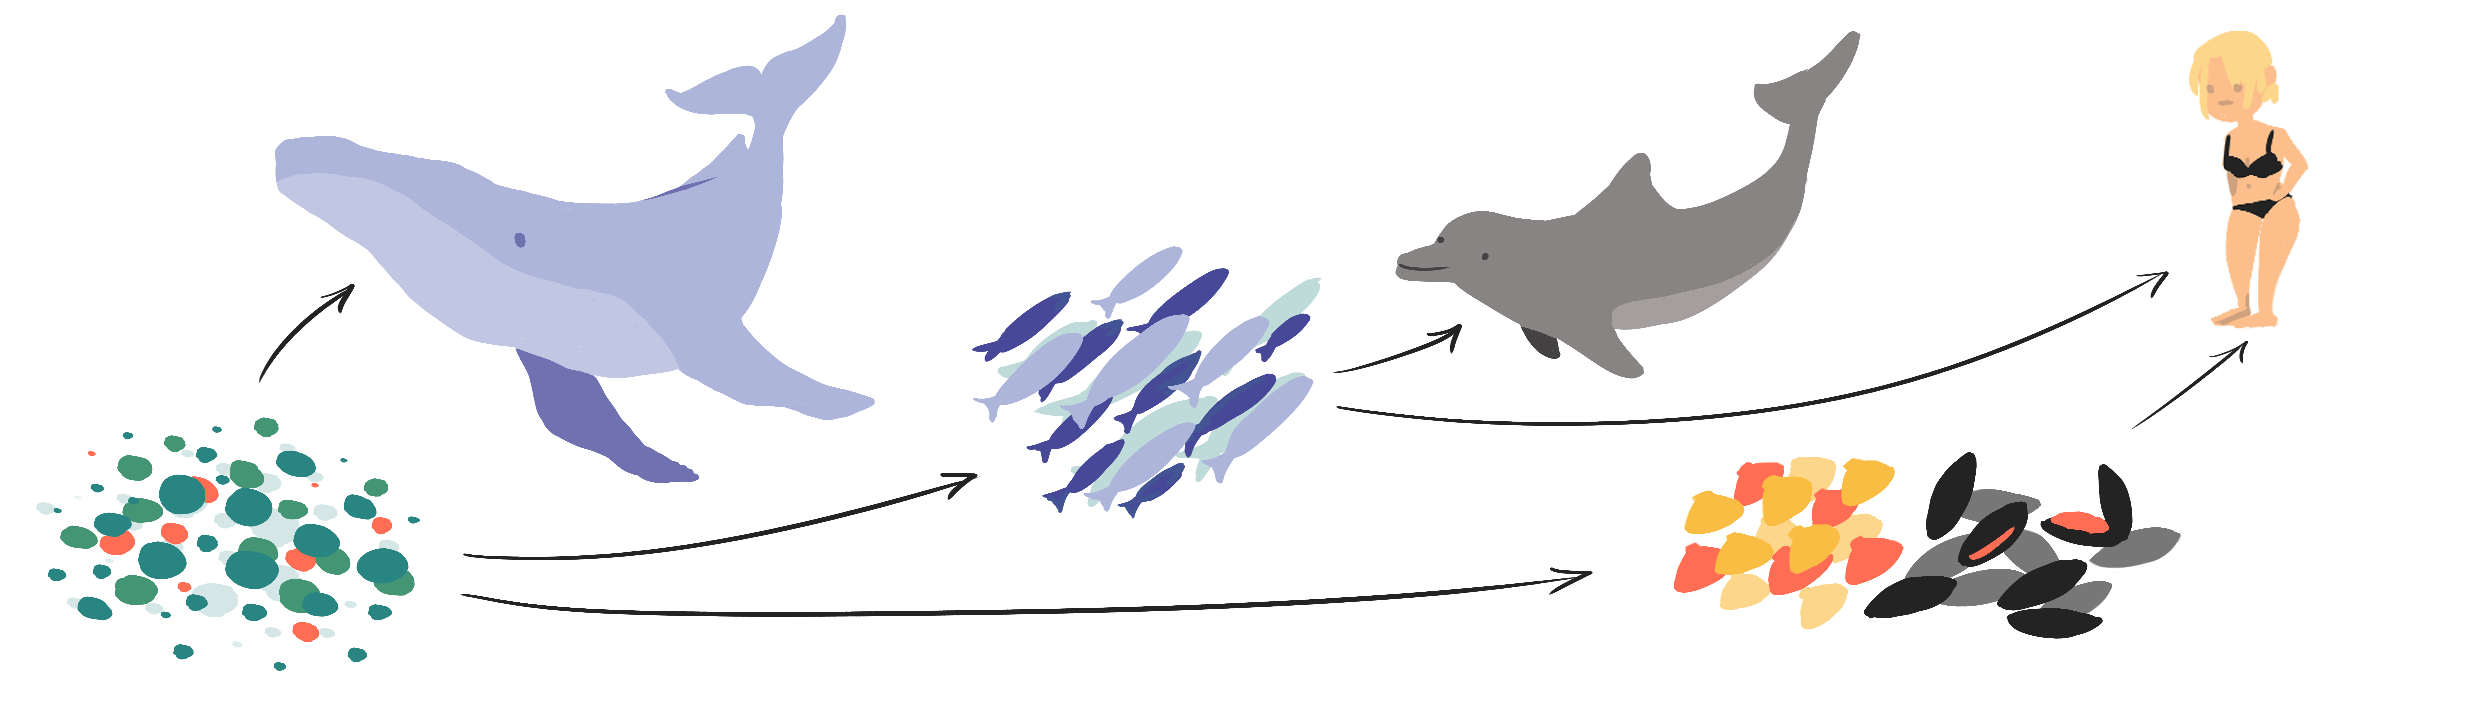
\includegraphics{food-chain}
    \caption[Marine toxins through the food chain]{Example of the advancement of marine toxins through the food chain by bioaccumulation}
    \labfig{food-chain}
\end{figure}

The most direct implication of this phenomenon lies in the seafood industry: when a harmful algal bloom occurs the mollusks that are being grown in the area become poisonous.
In order to prevent intoxications, the harvesting and selling has to be put on hold until the concentration of toxins in the water and in the seafood has gone down back to safe levels, with great economic losses for the fish market, the tourism industry and the restaurant business.\sidecite{hoagland02}

Specifically, STX is produced by phytoplanktons from the genera \genus{Alexandrium}, \genus{Gymnodinium} and \genus{Pyrodinium},\cite{gerssen10} as well as freshwater cyanobacteria bacteria including \genus{Anabaena} and \genus{Scytonema}.\cite{smith11,tebrineh10,}
When these species experience a bloom and free large quantities of STX into their ecosystem, bivalve organisms such as \genus{Mactridae}, \genus{Myacidae}, \genus{Mytilidae} and \genus{Veneridae} absorb it by filtration and accumulate it in their kidneys, feet and digestive glands\cite{oikawa05} until they reach hazardous concentrations.

Saxitoxin (STX), the protagonist of this introduction, is one of the substances that commonly become a threat when such blooms happen.
According to their chemical structure, marine toxins can be classified as domoic acid, saxitoxins, brevetoxins, okadaic acid, dinophysitoxins, pectenotoxins, yessotoxins, axaspiracids, spirolides and gymnodimines.\cite{gerssen10}\sidenote{STX, of course, belongs to the family of saxitoxins, but it's actually the head of a group with up to 57 different derivates.\cite{schantz75,bordner75,shimizu81}}

\begin{marginfigure}
    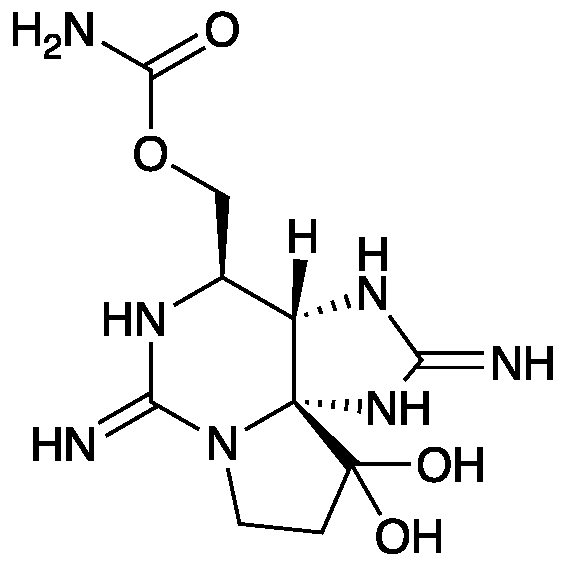
\includegraphics{stx-unlabeled}
    \caption[Structure of STX]{Structure of STX}
    \labfig{stx-unlabeled}
\end{marginfigure}

From a biological standpoint, STX is responsible for a human syndrome known as paralytic shellfish poisoning (PSP).
PSP involves the binding of the STX to the voltage gated sodium channels of the cells in the nervous systems, blocking the transmission of nervous impulses and effectively paralyzing the poisoned organism.
Specific symptoms of PSP in humans include numbness, headaches, dizziness, nausea, vomiting, diarrhea, weakness, temporal loss of vision, inability to breathe, and even death by respiratory paralysis.\cite{visciano16,gerssen10}
STX is such a potent neurotoxin, with an oral LD$_{50}$ for humans of only \SI{5.7}{\micro\gram\per\kilo\gram} of body weight,\cite{nguyen20} that is was considered and developed as a biochemical weapon by the United States in the past.\cite{stewart06}

For these reasons there exist health regulations, detection and quantification procedures that help identify algal blooms and regulate the seafood market.
Specifically, the standard procedure for the detection of STX is the mouse bioassay (MBA).
The MBA, which has a limit of quantification of around \SI{370}{\micro\gram\per\kilo\gram}\sidecite{efsa09} consists in injecting an extract of a contaminated organism into a mouse.
The concentration of toxin in the contaminated sample can be estimated by measuring the time from injection to death.\cite{who84}
Apart from the bioethical issues that are inherently tied to this methods, it's also subject of another controversy.
The current regulatory limits in the European Union are of \SI{800}{\micro\gram\per\kilo\gram}.
However, by following acute reference dose (ARfD) criteria, we find out that the limits should be actually of \SI{75}{\micro\gram\per\kilo\gram}.\sidenote{Which results when taking the acute dose of \SI{0.5}{\micro\gram\per\kilo\gram} of body weight, and considering a \SI{60}{\kilo\gram} adult eating a reference portion of \SI{400}{\gram} of shellfish.}\cite{efsa09}
While its quantification limits are low enough to comply with the current EU regulations, they are insufficient when taking into account realistic health criteria.

There are newer alternative methods that don't rely on animal testing.
One of them is liquid chromatography with fluorescence detection and has a limit of detection between \SI{10}{\micro\gram\per\kilo\gram} and \SI{80}{\micro\gram\per\kilo\gram}.\cite{eu17,aoac16}
This method, developed by AOAC, is used as a co-official technique in the European union and has a good sensibility, but involves a series of derivatization steps and is time consuming.
Other common tests are enzime-linked inmunnosorbent assays\sidenote{More commonly known by their acronym ELISA}, which have a limit of detection of about \SI{0.015}{\nano\gram\per\litre}.\cite{wharton17}
These are not reliable or sensible enough to be used for quantification, and are often relegated to screening purposes.

The aim of this work in the context of the problem at hand, therefore, is to find realistic proposals for a better and more convenient method to identify and quantify STX.
To do this, the main focus of the research is put on spectroscopy.

\section{The work up until now}
\labsec{previous-work}

The author's involvement in finding appropriate spectroscopic techniques and environments for the detection of SXT dates back to previous work.
The efforts began with its computational characterization: modelling the STX, studying its acid-base behavior, assessing its conformational freedom in order to find its predominant structures...
After this preliminary treatment, several spectroscopic techniques were simulated and evaluated.

As a general approximation to vibrational spectroscopy, the vibrational normal modes were calculated and individually assessed in order to select a set of modes that, when present in a spectrum as peaks, could be used to unequivocally identify STX.
These modes could be visible in Infrared (IR) spectra, in Raman spectra, or in both.

IR spectroscopy was the first that was tested.
Vibrational modes are active in IR if by virtue of they symmetry they affect the dipole moment of a molecule.
The IR spectrum of the isolated STX was decently clear, and a good part of its characteristic vibrational modes were visible.
However, we had to take into account the fact that real life samples would consist mainly of seawater.
Water is very active in IR spectroscopy, with an ample signal between \SI{3500}{\per\cm} and \SI{4000}{\per\cm} due to stretchings, and a scissoring peak at \SI{1600}{\per\cm}.
These signals, with intensities proportional to the much higher quantities of water, would obscure those of the dilute STX, located near those same frequencies.
Extracting the STX from the water and redissolving it into a different solvent could be a way to fix this issue and make use of IR, but it would imply additional time and cost.

Water, however, has very weak signals in Raman.
Raman spectroscopy is able to detect vibrational modes that have an effect on the polarizability of a molecule.
This kind of spectroscopic technique relies on the effect of Raman scattering: a phenomenon in which the photons of a laser interact inelastically with molecular vibrations resulting in their energy being shifted up or down.
After generating Raman spectra for the STX, it was decided that the Raman active modes and their corresponding peaks would be sufficient to clearly identify the toxin.
There just remained the issue of the intensity: the Raman scattering effect has a very low probability, which in a real spectrum translates into very low intensities that could easily get obscured by the noise from the signals of other molecules.
For this reason, the Raman spectroscopy had to be coupled with at least one amplification technique that could selectively amplify the signals related to STX.

The method chosen for this purpose was resonance Raman (RR).
While more about this effect and its fundamentals can be read in \refsec{rr-methods}, the practical simulation of RR can be summarized as \q{tuning the frequency of a laser so that the Raman scattering excitation coincides with an electronic transition}.
The problem with this approach was the following: while STX certainly benefits from resonance effects and Raman spectra with great amplifications can be generates, all of its electronic transitions are located below \SI{200}{\nano\metre}.
In a real life setting, it would be prohibitively expensive and dangerously energetic to use lasers of such small wavelengths: the most common lasers for RR range between \SI{244}{\nano\metre} and \SI{1064}{\nano\metre}, where the most common ones tend to be around the visible and near-infrared wavelengths.\cite{karlsson18,horiba}
Since this work aims to propose feasible and practical ideas, we had to find a way to modify STX's natural range of absorption.
The answer lied close to the fundamentals of another Raman amplification technique: surface-enhanced Raman spectroscopy (SERS).
SERS is a variant of Raman that relies on the adsorption of a molecule onto a surface-like structure, usually composed of a metal.
While the Raman signal amplification was notable, the most interesting result that we found while studying SERS was the fact that adsorbing the STX to another molecule modified its electronic properties\sidenote{Resulting in what could be thought of as the shared electronic properties of a complex.} in such a way that its UV-vis absorption range was shifted towards larger wavelenghts.

The system with which this effect was initially studied in previous work was a graphene sheet.
While the graphene-STX complex was successful in absorbing wavelengths longer than STX alone, it was found that the vibrations of the surface interfered with the identification of the molecule.

In this work, then, we intend to keep exploring that last idea: the binding of STX to another surface-like molecule with the aim of improving its electronic properties.
To continue the research along these lines would imply the selection of promising surface-like molecules, the characterization of the properties and spectroscopy of said molecules, and the study of their interactions with STX.


\section{The sunflower molecules: introduction and origin}

\begin{marginfigure}
    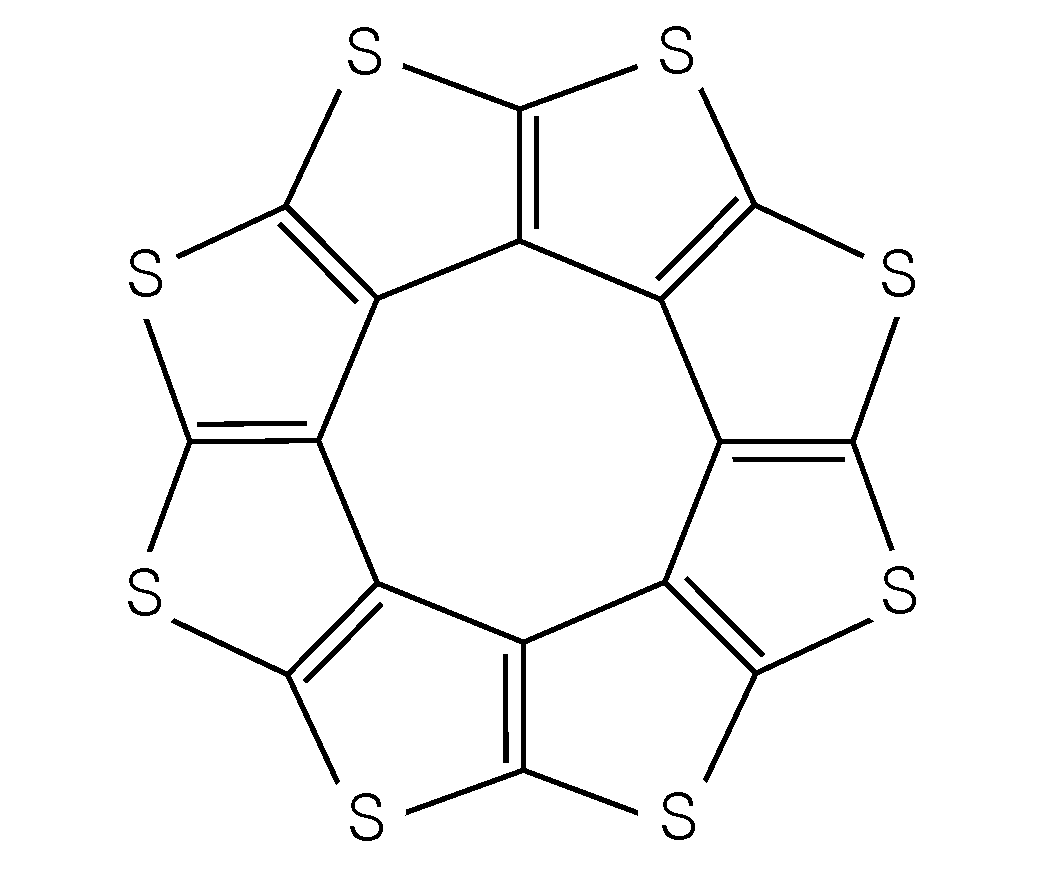
\includegraphics{sulflower-structure}
    \caption[Structure of sulflower]{Structure of sulflower}
    \labfig{sulflower-structure}
\end{marginfigure}

The search for effective and interesting SERS substrates ended up leading us to a novel class of molecules researched and presented in the year 2006 by Chernichenko and his colleagues.\sidecite{chernichenko06}
The first representative of this family, nicknamed as \q{sulflower}, is the ocatathio[8]circulene.
This highly symmetric structure, which may be described as a form of carbon sulfide and as a belt of annulated thiophene cycles, is claimed to have great stability, high symmetry and unusual electronic properties.

From a synthetic point of view, sulflower also proved to be simple and straightforward to develop despite its complex appearance: start from tetrathiophene, sulphurize its free sites and acidificating to get polythiol, and remove the excess sulfur by vacuum pyrolysis.
This process allowed the team to achieve yields of 56\% starting from commercially available reagents.

Interestingly, the team proposed that it could be possible to prepare materials with diverse electronic properties by using different types of heteroatoms and varying on the basic structure of the molecule.
Such a statement made apparent the potential of this family of molecules: highly symmetrical, stable, surface-like structures with variable electronic behavior could act as suitable substrates for Raman amplification.
\refch{sunflowers} will be entirely dedicated to that premise: the study and characterization of sulflower and sulflower-like molecules, which from now on I will collectively refer to as \q{sunflowers} or simply \q{flowers}.
By designing, generating and studying our own family of sunflowers, we will be contributing to the characterization of a novel and interesting group of molecules, and we may be able to identify an ideal resonance Raman and SERS environment for STX.
Before that, however, a technical word on computational methods, calculation level, software and hardware.
